\section{Non-Adaptive Experiments}\label{sec:model}
In this section, we study the \cmtfinal{staggered rollout} design of non-adaptive experiments. In Section \ref{subsec:estimator}, we present an approach for estimating $\tau_0, \tau_1, \cdots, \tau_\ell$.  Next, in Section \ref{subsec:objective}, we define the precision of the proposed estimators. We formulate an optimization problem, where for a given estimator, the solution yields the set of treatment times for each unit that maximizes the precision of the estimator. Finally, we present our solution to the optimization problem in Section \ref{subsec:result-carryover}.

 \subsection{Estimation of Instantaneous and Lagged Effects}\label{subsec:estimator}
    The decision maker needs to consider two objectives when choosing an estimator for $\tau_0, \tau_1, \cdots, \tau_\ell$. First is the statistical properties of this estimator, such as the bias, variance, and mean-squared error (MSE). Second is the feasibility of optimizing units' treatment times based on the properties of this estimator. For example, one can study the optimal treatment assignments based on MSE of a simple estimator \cmtrx{such as the difference-in-means estimator}, but this simple estimator can have a large \cmtrx{variance and} MSE. Alternatively, one can use a sophisticated estimator with a small MSE \cmtrx{such as regularized matrix factorization estimator in Section \ref{sec:algorithm}}, but the functional form of MSE may be very complex, which can lead to an intractable optimization problem in the design phase.

    In this paper, we seek to balance these two objectives. We study the optimization of treatment assignments, for a particular estimator, namely the Generalized Least Squares (GLS) estimator, given a particular model for the data generating process. The GLS estimator for $\tau_0, \tau_1, \cdots, \tau_\ell$ is based on  the following specification
    %
    \begin{equation}\label{eqn:model-setup} 
    Y_{it} = \alpha_i +  \beta_t + \*X_i^\T  \bm{\theta}_t + \tau_0 z_{it} + \tau_1 z_{i,t-1} + \cdots + \tau_{\ell} z_{i,t-\ell}  + \underbrace{\*u_i^\T \*v_t + \varepsilon_{it}}_{e_{it}}\, ,
    \end{equation}
	where $\alpha_i$ and $\beta_t$ are unobserved unit and time fixed effects, $\*X_i  \in \+R^{d_x}$ are observed covariates of dimension $d_x$, $\bm{\theta}_t \in\+R^{d_x}$ are their (non-random) unobserved time-varying coefficients $\bm{\theta}_t$, $\*u_i \in \+R^{d_u}$ are latent (non-random) covariates of dimension $d_u$, $\*v_t \in \+R^{d_u}$ are (random) latent factors, and $\{\varepsilon_{it}\}_{it\in[N]\times[T]}$ are unobserved residuals. We allow $d_x = 0$, that is, \eqref{eqn:model-setup} does not have observed covariates. We also allow $d_u = 0$, that is, \eqref{eqn:model-setup} does not have latent covariates.
	

The specification with two-way ({\it i.e.}, unit and time) fixed effects and possibly with observed covariates has been widely used in observational studies to estimate treatment effects \citep{angrist2008mostly}.\footnote{There are two reasons. First, $\alpha_i$ and $\beta_t$ can be arbitrarily correlated with the observed explanatory variables $(\*X_i, {z}_{it}, \cdots, {z}_{i,t-\ell})$, so they can capture the unobserved additive unit-specific and time-specific confounders that jointly affect ${z}_{it}$ and $Y_{it}$ \citep{angrist2008mostly}. Second, $\alpha_i$ captures the mean effect of unobservables on unit $i$'s outcome over time, and $\beta_t$ captures the mean effect of unobservables on units' outcomes at time $t$. } Observed covariates $\*X_i$ in \eqref{eqn:model-setup} are time-invariant and are not affected by the treatment. Examples of such covariates are an individual's gender and race or attributes of a city.\footnote{The time-invariance assumption is commonly used in difference-in-differences estimators \citep{card1994minimum} 
% \citep{heckman1997matching,heckman1998matching,blundell2004evaluating,abadie2005semiparametric}
and synthetic control estimators \citep{abadie2010synthetic} in observational studies.} Using $\alpha_i$, $\beta_t$ and $\*X_i$ controls for the heterogeneity in units and time periods, that can effectively reduce variance in treatment effect estimation. Note that \eqref{eqn:model-setup} has the interactive latent factor structure $\*u_i^\T \*v_t$ that can capture the multiplicative unobserved effects, and is therefore more general than the specification with additive effects $\alpha_i$ and $\beta_t$ only. \cmtrx{We assume $\*v_t$ is random, but $\*u_i$ is nonrandom for the design purpose. Such an assumption is also imposed in a different literature that estimates the latent factors on large panels  \citep{bai2002determining,bai2003inferential}. }

    	GLS estimates $\tau_0, \cdots, \tau_\ell$, $\alpha_i$, $\beta_t$ and $\bm{\theta}_t$ by minimizing the weighted sum of squared residuals $e_{it}$ in \eqref{eqn:model-setup} (see Section \ref{subsec:gls-carryover} for more details). GLS has two nice properties \cmtfinal{when the optimal weights are chosen, following} the Gauss-Markov Theorem (see Lemma \ref{lemma:gauss-markov} in Section \ref{subsec:gls-carryover}) under the strict exogeneity assumption in Assumption \ref{ass:constant-error} below. First, GLS is the best linear unbiased estimator (BLUE) of $\tau_0, \cdots, \tau_\ell$, meaning that this estimator has the smallest variance among all the linear unbiased estimators. Second, there is an explicit formula for the variance and precision of GLS in terms of $z_{it}$, which makes the treatment design problem tractable. 
	
	
	\begin{assumption}[Error Structure]\label{ass:constant-error}
	\cmtrx{$\*v_t \in \+R^{d_u}$ is i.i.d. in $t$}
 with  $\+E[\*v_t  \mid \bm{\xi}_{it}] = \bm{0}$ and $\+E[\*v_t \*v_s^\T \mid \bm{\xi}_{it}, \bm{\xi}_{js} ] = \bm\Sigma_{v} \cdot \bm{1}_{t = s}$ for all $i, j, t$ and $s$, where $\bm{\xi}_{it} = (\*X_i, z_{it}, \cdots, z_{i-\ell, t})$. Moreover, $\varepsilon_{it} $ is i.i.d. in $i$ and $t$ with $\+E[\varepsilon_{it} \mid \bm{\xi}_{it}] =0$ and $\+E[\varepsilon_{it} \varepsilon_{js}  \mid \bm{\xi}_{it}, \bm{\xi}_{js} ] = \sigma_\varepsilon^2 \cdot \bm{1}_{i = j, t = s}$ for all $i, j, t$ and $s$. In addition, $\varepsilon_{it}$ is independent of $\*v_s$  for all $i, t$ and $s$.
	\end{assumption}

	
	\begin{remark}[Machine learning heuristics for $\bm{\tau}$]
	    Instead of focusing on the least squares estimator, one can look at other estimators, for example, machine learning estimators.
	    We provide one such estimator in Section \ref{sec:algorithm} for $\bm{\tau}$ that does not rely on Assumption \ref{ass:constant-error} about $\*v_t$. This type of machine learning-based estimators are typically biased in the estimation of $\bm{\tau}$, but could have a smaller variance than the unbiased estimators. The optimization of $Z$ based on these estimators is generally not tractable, and therefore we do not emphasize them in this paper.
	\end{remark}
	
	
		\begin{remark}[Implication of Assumption \ref{ass:constant-error}]
	$\+E[\*v_t] = 0$ holds without loss of generality, as we can always project their mean to $\alpha_i$.\footnote{If $\+E[\*v_t] \neq 0$, let $\alpha^\dagger_i = \alpha_i + \*u_i^\T \+E[\*v_t] $ and $\*v^\dagger_t = \*v_t - \+E[\*v_t]$, and then $\*v^\dagger_t $ has mean zero. } 
	Under Assumption \ref{ass:constant-error}, $e_{it}$ satisfies 
	\[\+E[e_{it}] = 0, \qquad \+E[e_{it}^2] = \*u_i^\T \*\Sigma_{v} \*u_i + \sigma_{\varepsilon}^2, \qquad \+E[e_{it} e_{jt}] = \*u_i^\T \*\Sigma_{v} \*u_j, \qquad \+E[e_{it}e_{js}] = 0, \quad \text{ for } \,\, t \neq s, \]
	implying that $e_{it}$ is correlated in the unit dimension, but it is uncorrelated in the time dimension.
	\end{remark}
%
\cmtfinal{\begin{remark}[Feasiblity of GLS]
     The weight matrix $\*W$ in GLS is optimal when it is proportional to the inverse covariance matrix of $\bm{e}_t = [e_{it}]_{i \in [N]}$, {\it i.e.}, $\big(\*U \*\Sigma_v \*U^\T + \sigma_\varepsilon^2 \*I_N \big)^\I $ with $\*U = [\*u_i]_{i \in [N]}$. As the optimal weight matrix is unknown, in practice, we can use feasible GLS, where we first use OLS, estimate the optimal weight matrix, and then use GLS with the estimated weight matrix. 
 \end{remark}
 }
 
	
	    \begin{remark}[Treatment Effect Estimation with Heterogeneity]\label{rem:hetreogeneous}
    Specifications like \eqref{eqn:model-setup} have been commonly used to estimate average treatment effects in empirical studies in many domains, such as economics \citep{card1994minimum}, operations ({\it e.g.}, \cite{cui2019learning,cachon2019does}),
    % \citep{cui2019learning,cachon2019does,cui2020sooner,zhang2020long}
    and healthcare \citep{abaluck2021impact}. Such specifications do not restrict treatment effects to be homogeneous. In Remark \ref{remark:cate} below, we discuss an alternative estimation approach when heterogeneous treatment effects are the objects of interest.
	\end{remark}
	

	% \tocless
 \subsection{Optimization Problems for Treatment Decisions}\label{subsec:objective}
	
	In this section, we introduce the optimization problem to solve the optimal $Z$ based on the statistical properties of GLS. From a high level perspective, we are interested in precisely estimating $\bm{\tau}$. However, there are $\ell+1$ parameters in $\bm{\tau}$ and it is generally infeasible to find an $Z$ that simultaneously maximizes the precision of each of $\hat{\tau}_0, \cdots, \hat{\tau}_{\ell}$ for $\ell \geq 1$. Instead, one needs to consider an objective function that summarizes the precision of each of $\hat{\tau}_0, \cdots, \hat{\tau}_{\ell}$ into a scalar. There are two categories of objective functions that one may be interested in:
	\begin{itemize}
	    \item Balancing the precision/variance of each of $\hat{\tau}_0, \cdots, \hat{\tau}_{\ell}$
	    \item Maximizing the precision of some linear combination of $\hat{\tau}_0, \cdots, \hat{\tau}_{\ell}$
	\end{itemize}
	Examples of the objective functions related to the first category include \citep{atkinson2007optimum} 
	\begin{itemize}
	    \item \textbf{A-optimal design}: minimizes the trace of $\var(\hat{\bm{\tau}})$
	    \item \textbf{D-optimal design}: minimizes the determinant of $\var(\hat{\bm{\tau}})$
	    \item \textbf{T-optimal design}: maximizes the trace of the inverse of $\var(\hat{\bm{\tau}})$
	\end{itemize}
	An example of the objective functions related to the second category is
\begin{itemize}
    \item \textbf{Cumulative effect} ($\sum_{j=0}^\ell \tau_j$): minimizes $\var\big(\sum_{j = 0}^\ell \hat{\tau}_j\big)$
\end{itemize}


% \textcolor{red}{\bf (should we hint in the introduction that what we do is look at a a linear combination of variances, or the variance of a linear combination, when we first mention that we look at different objects, eg various lagged effects?)} \cmtrx{RX: added a sentence in the introduction.}

    When $\ell = 0$, the four objective functions mentioned above are equivalent to one another. For general $\ell$, they are not equivalent, and the optimal treatment assignments for these four objectives can be different (but the difference
can be small). 

    In this section, we focus on finding the optimal assignment
    $A = [A_i]_{i \in [N]}$, where $A_i \in [T] \cup \{\infty\}$ denotes the first time that unit $i$ adopts the treatment ($A_i=\infty$ means unit $i$ was never treated\footnote{We use ``$\infty$'' to preserve the ordering that a larger value for $A_i$ implies the treatment is assigned at a later time.}). Because the treatment is irreversible, there is a one-to-one mapping between $(z_{i1}, z_{i2}, \cdots, z_{iT})$ and $A_i$. Given the reduction to the $N$ adoption times we focus on
    analytically solving the T-optimal (or trace-optimal) design:
	 \begin{equation}\label{eqn:obj}
 \cmtrx{\max_{A}  \tr \big(\mathrm{Prec}(\hat{\bm{\tau}}; A)  \big)  ,}
	\end{equation}
 \cmtrx{where $\mathrm{Prec}(\hat{\bm{\tau}}; A)$ is the precision matrix of $\bm{\tau}$ and is defined as the matrix inverse of the variance-covariance matrix of $\bm{\tau}$, $\var(\hat{\bm{\tau}}; A)$, when the assignment $A$ is used.}
	% where $\mathrm{Prec}(\hat{\bm{\tau}})$ is the precision matrix of $\bm{\tau}$ and is defined as the matrix inverse of $\var(\hat{\bm{\tau}})$
	
% \textcolor{red}{\bf (may be write Prec explicitly as a function of the fraction treated in each period, that is, as  a function of $A$.)}

	T-optimal design was first introduced by \cite{atkinson1975design} to discriminate between two competing regression models ({\it e.g.}, to determine whether $\ell = \ell_0$ or $\ell = \ell_1$ is true, for distinct number of lags $\ell_0$ and $\ell_1$ in our setting). Since then, the T-optimal design has been studied by \cite{atkinson1975optimal,ucinski2005t,wiens2009robust,dette2012t,dette2013robust,dette2015bayesian} and others.  
	
	Solving the T-optimal design is generally challenging, even in some special cases (see Example \ref{example:T-1-ell-0}).
	We provide the explicit optimality conditions for the integer program \eqref{eqn:obj} in Section \ref{subsec:result-carryover}. Based on the optimality conditions, we provide an algorithm on choosing a design in Algorithm \ref{algo:choose-design} in Section \ref{subsubsec:estimate-latent-covariates}. 
	Admittedly, the other three objectives mentioned above would be natural and of practical interest, especially the one that minimizes the variance of the estimated cumulative effect, $\var\big(\sum_{j = 0}^\ell \hat{\tau}_j\big)$. However, analytically solving the other three objectives is generally infeasible, as explained in Remark \ref{rem:alternative-objectives} below. Instead, one could numerically solve the other three objectives in practice. We visualize the numerical solutions for D-optimal design in Figure \ref{fig:carryover-treatment-effect-d-opt} in Section \ref{subsec:d-optimal-design}, which has a similar structure as our solutions to \eqref{eqn:obj}. We empirically show in Section \ref{sec:empirical} and Section \ref{subsubsec:robustness-to-alternative-metrics} that our solutions to \eqref{eqn:obj} outperform the benchmark treatment designs measured by the objective of A-optimal design and $\var\big(\sum_{j = 0}^\ell \hat{\tau}_j\big)$.
	

	

	\begin{example}\label{example:T-1-ell-0}
	    If $T=1$, $\ell = 0$, and all the covariates are observed ({\it i.e.}, $d_u = 0$),  \eqref{eqn:obj} coincides with the offline optimization problem in \cite{bhat2019near}, and is equivalent to the MAX-CUT problem and is NP-hard \citep{hayes2002computing,mertens2006easiest}. In this paper, we focus on the case of low-dimensional covariates.\footnote{This makes sense as we allow for latent covariates, which can summarize the information and reduce the dimensionality of (high-dimensional) observed covariates.} Our solution from Algorithm \ref{algo:choose-design} is provably close to the optimal integer solution to \eqref{eqn:obj} for a large $N$. 
	\end{example}
	


    \begin{remark}[Challenges in alternative objectives]\label{rem:alternative-objectives}
    Note that each entry in $\var(\hat{\bm{\tau}}) $ is a ratio of two polynomial functions of $z_{it}$, where the degrees of numerator and denominator are $2\ell$ and $2(\ell+1)$, respectively, for $\ell \geq 1$. The objective of A-optimal design and $\var\big(\sum_{j = 0}^\ell \hat{\tau}_j\big)$ are both sums of entries in $\var(\hat{\bm{\tau}}) $ ({\it i.e.}, sums of ratios of two higher-order polynomials of $z_{it}$). The objective of D-optimal design is the inverse of a $2(\ell+1)$-th order polynomial function of $z_{it}$. \cmtfinal{The objective functions of both A-optimal and D-optimal design are non-convex. Therefore, using the first order condition only is generally not sufficient to solve the global optimal solution.}
 	\end{remark}
 	
 	

	{\blue 
	% \tocless
 \subsection{Optimal Solutions}\label{subsec:result-carryover}
	We provide the optimality conditions for the T-optimal design. The optimality conditions disentangle the effect of different components in \eqref{eqn:model-setup} ({\it i.e.}, two-way fixed effects, observed and latent covariates) on the optimal treatment assignments. This problem is challenging in our setting with multiple units and periods for two reasons. First, different components can potentially affect the optimal design in both unit and time dimensions. Second, the effect of different components may be convoluted and interact with one another.
	
	To build intuition, we start with the solution to a simple specification.
	
	\begin{example}[Two-way fixed effects and $\ell = 0$]\label{example:two-way-fe}
	Suppose $Y_{it} = \alpha_i + \beta_t + \tau_0 z_{it} + \varepsilon_{it}$, and and Assumptions \ref{ass:treatment-adoption}, \ref{ass:model}, and \ref{ass:constant-error} hold. Then the objective function in \eqref{eqn:obj} equals to
\begin{align}\label{eqn:precision-ell-0}
      \mathrm{Prec}(\hat{\tau}_0; A)
    = \frac{N}{\sigma_\varepsilon^2 } \left[ - 2 \bm{b}_T^\T \bm{\omega} -\bm{\omega}^\T \*P_{\bm{1}_{T}} \bm{\omega} \right],
\end{align}
which is a quadratic and concave function of $\bm{\omega} = [\omega_t]_{t \in [T]}$ with $\omega_t = N^{-1} \sum_{i=1}^N z_{it}$, $\*P_{\bm{1}_{T}} = \*I_{T} - \bm{1}_{T} \bm{1}_{T}^\T/T$, and $\*b_T = [b_{t}]$ with $b_{t} = (T+1-2t)/T$. By solving the first-order condition, we can show that any treatment design satisfying
${\omega}^{\ast}_t = -b_t$ for all $t$ is optimal and maximizes the precision. In the optimal solution,  the treated fraction is linear in time. This result is conceptually similar to those in \cite{lawrie2015optimal,girling2016statistical,li2018optimal} that show the optimal treated fraction is linear in time, under a similar specification, but with $\alpha_i$ to be random effects. More intuition for the linear treated fraction is provided in Section \ref{subsec:treated-fraction}. 



	\end{example}
	
	

Next consider a more general specification with $\ell > 0$, but without $\*X_i$ or $\*u_i$. We can show the objective function in \eqref{eqn:obj} is still quadratic and concave in $\bm{\omega}$, but takes a more complicated form (see Lemma \ref{lemma:simplify-obj} in Section \ref{subsec:separate-quadratic}), leading to nonlinear optimal treated fraction in time. Specifically in Theorem \ref{thm:obs-latent-carryover-model} we show that in the optimal solution, the unit average of $z_{it}$ satisfies 
%
		\begin{equation}\label{eqn:omega-carryover}
		\omega_{\ell,t}^\ast = \begin{cases}
		-1 & t \leq \lfloor \ell/2 \rfloor \\
		a^{(\ell)}_{t-\lfloor \ell/2 \rfloor} & \lfloor \ell/2 \rfloor < t \leq \ell \\
		-1 + \big(2t - (\ell+1)\big)/(T - \ell)  & \ell < t \leq T - \ell \\
		- \omega^\ast_{\ell,T+1-t} & T - \ell <  t \leq T-\lfloor \ell/2 \rfloor \\
% 		- ((M^{(\ell)})^{-1} b^{(\ell)} )_{T+1-\lfloor \ell/2 \rfloor-t} & T - \ell <  t \leq T-\lfloor \ell/2 \rfloor \\
		1 & T-\lfloor \ell/2 \rfloor < t \\
		\end{cases}
		\end{equation}
		where $a^{(\ell)}$ is a vector of length $\ell - \lfloor \ell/2 \rfloor$ defined in Section \ref{subsec:def-A-l-B-l}. $\omega_{\ell,t}^\ast$ has five stages and follows an $S$-shaped curve in time $t$: stage 1:  all units are under control; stage 2: $\omega_t^\ast$ grows non-linearly in time (because of $a^{(\ell)}$); stage 3: $\omega_t^\ast$ grows linearly in time; stage 4: $\omega_t^\ast$ grows non-linearly in time again; stage 5, all units are under treatment. The optimal solution is symmetric with respect to the center ({\it i.e.}, $\left((T+1)/2, 0 \right)$). Figure \ref{fig:carryover-treatment-effect-t-opt} demonstrates $\omega_{\ell,t}^\ast$ for various $\ell$ in a $T=12$ period problem.  More examples of $\omega_{\ell,t}^\ast$ will be provided in Section \ref{subsec:treated-fraction}.
		
	Furthermore, suppose the specification contains at least one of the $\*X_i$ or $\*u_i$ components. A commonly used variance reduction approach in cross-sectional studies is to balance covariates, so that treated and control units are comparable when the two groups have similar covariates ({\it e.g.}, \cite{imbens2015causal}).\footnote{There is a strand of literature in operations research to use discrete optimization to achieve covariate balancing \citep{nikolaev2013balance,bertsimas2015power,bertsimas2019covariate,bhat2019near}, and to use stratified sampling to increase power \citep{fox2000separability,mulvey1983multivariate}.} Similar intuition carries over to the panel setting. We show in Theorem \ref{thm:obs-latent-carryover-model} below that the optimal design balances covariates groups, where groups are defined as the set of units with the same initial treatment time. 
	
	
	We state the first of our main theorems using the following solution concepts: Let $\mathbb{A}_{\ell} = \big\{ A:  N^{-1} \sum_{i = 1}^N \boldsymbol{1}_{A_i \leq t}  = (1+\omega_{\ell,t}^\ast)/2,\, \forall t\big\}$ be the set of designs satisfying \eqref{eqn:omega-carryover}. When $d_x > 0$, let $\mathbb{A}_{\*X} =  \big\{ A: N^{-1} \sum_{i = 1}^N  \*X_i \boldsymbol{1}_{A_i  =  t}  = \bm{0}_{d_x},\, \forall t \in \{2,\cdots,T\}\big\}$ be the set of designs satisfying covariate balancing conditions (suppose rows in $\*X = [\*X_i]_{i \in [N]}$ are centered). When $d_x = 0$, let $\mathbb{A}_{\*X} = \mathbb{A}^N$ and no conditions need to be imposed related to $\*X_i$. $\mathbb{A}_{\*U}$ is defined similarly as $\mathbb{A}_{\*X}$.
	}
	

		\begin{theorem}[Optimality Conditions]\label{thm:obs-latent-carryover-model}
		Suppose Assumptions \ref{ass:treatment-adoption}, \ref{ass:model}, and \ref{ass:constant-error} hold, $\hat{\bm{\tau}} $ is \cmtrx{estimated from the infeasible GLS}
		% \textcolor{red}{(\bf this is the infeasible GLS)}
		with $\*W \propto \big(\*U \*\Sigma_v \*U^\T + \sigma_\varepsilon^2 \*I_N \big)^\I $,  rows in $\*X$ and $\*U$ are centered $($i.e., $\sum_{i = 1}^N \*X_i = \bm{0}_{d_x}$ and $\sum_{i = 1}^N \*u_i = \bm{0}_{d_u}$$)$, $\*X$ and $\*U$ are orthogonal $($i.e., $\sum_{i = 1}^N \*X_i \*u_i^\T = \mathbf{0}_{d_x \times d_u}$$)$, $\*\Sigma_v = \sigma_\varepsilon^2 \cdot \*I_{d_u}$, and $T > (\ell^3+13\ell^2+7\ell+3)/(8\ell)$.
		 $A$ is an optimal treatment design if $A  \in \mathbb{A}_{\mathrm{opt}} $, where 
		\begin{equation}\label{eqn:carryover-t-optimal-obs-latent-thm}
		\mathbb{A}_{\mathrm{opt}} = \mathbb{A}_{\ell}  \cap \mathbb{A}_{\*X} \cap \mathbb{A}_{\*U}\, .
		\end{equation}
		%
	\end{theorem}
	
	
	\begin{figure}[t!]
		\centering
		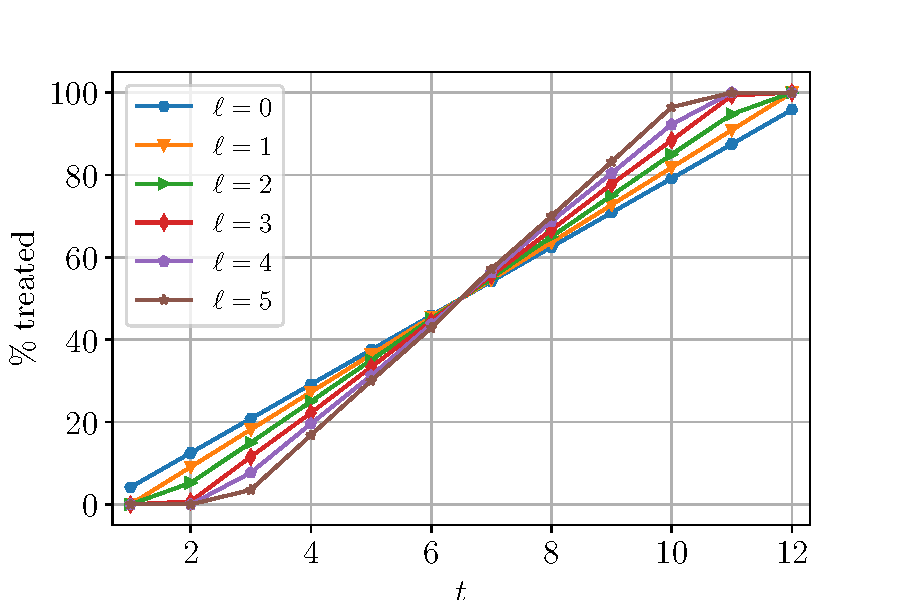
\includegraphics[width=0.4\linewidth]{plots/illustration/carryover-t-optimal.pdf}
		\caption{\textbf{{T}-optimal design.} Optimal treated fraction in the design of 12-period non-adaptive experiments with varying $\ell$. }
		\label{fig:carryover-treatment-effect-t-opt}
	\end{figure}
	
	Theorem \ref{thm:obs-latent-carryover-model} provides the optimality conditions for the T-optimal design when $\tau_0, \cdots, \tau_\ell$ are estimated from GLS using specification \eqref{eqn:model-setup}. The presence of $\alpha_i$ and $\beta_t$ makes the optimal treated fraction grow gradually over time, and the growth rate is determined by $\ell$. We further illustrate how the optimal treated fractions depend on $\alpha_i$, $\beta_t$, and $\ell$ in Section \ref{subsec:treated-fraction}. The presence of $\*X_i$ and $\*u_i$ imposes additional covariate balancing conditions, that can be satisfied if units in each stratum satisfy treated fraction conditions. Here strata are defined as groups of units with the same covariate value.  When covariates are discrete-valued, Example \ref{example:discrete-covariate} below provides a solution that satisfies the optimality conditions. For general cases, we provide guidance on choosing a design based on Theorem \ref{thm:obs-latent-carryover-model} in Section \ref{subsec:choose-a-design}.
\cmtrx{\begin{example}[Discrete $\*X_i$ and $\*u_i$]\label{example:discrete-covariate}
     Suppose $(\*X_i, \*u_i)$ is discrete and can only take $G$ values for a finite $G > 0$, denoted as $\{(x_g, u_g)\}_{g=1}^G$, each with positive probability. Then any $A$ in $\mathbb{A}^{\mathrm{disc}}_{\mathrm{opt}}$ defined below is in $\mathbb{A}_{\mathrm{opt}}$
		\begin{equation}\label{eqn:opt-finite-x-interactive-effect-carryover}
		\mathbb{A}^{\mathrm{disc}}_{\mathrm{opt}} =\bigg\lbrace A: \frac{1}{|\tlo_g|} \sum_{i \in \tlo_g} \boldsymbol{1}_{A_i \leq t}  = \frac{1+\omega_{\ell,t}^\ast}{2}  \,\,\,\, \forall t, g \bigg\rbrace\,,
		\end{equation}
		where $\tlo_g = \{i: (\*X_i, \*u_i) = (x_g, u_{g})\}$.
 \end{example}}
	
    \begin{remark}[Assumptions in Theorem \ref{thm:obs-latent-carryover-model}]
    The assumptions in Theorem \ref{thm:obs-latent-carryover-model} are non-restrictive for the following four reasons. 
	First, the assumption that rows in $\*X$ and $\*U$ are demeaned can be satisfied by projecting the mean onto the unit fixed effects $\bm{\alpha}$. Second, the assumption that $\*X$ and $\*U$ are orthogonal can be satisfied by applying the Gram-Schmidt procedure ({\it i.e.}, QR decomposition) to $\begin{bmatrix}
	 \*X & \*U \end{bmatrix}$ (which is possible as $\bm{\theta}$ is unknown and unrestricted). Third, $\*\Sigma_v = \sigma_\varepsilon^2 \cdot \*I_{d_u}$ is essentially an identification assumption, so that we can uniquely identify $\*u_i$ and $\*v_t$.\footnote{In other words, for arbitrary $\*u_i$ and $\*v_t$, we can right multiply $\*u_i^\T$ by $\sigma_\varepsilon \cdot \*\Sigma_v^{-1/2}$ and left multiply  $\*v_t$ by $\sigma_\varepsilon \cdot \*\Sigma_v^{-1/2}$ so that $v_t$ has variance $\sigma_\varepsilon^2 \cdot \*I_{d_u}$ (conditions $\sum_{i = 1}^N \*u_i = \bm{0}_{d_x}$ and  $\sum_{i = 1}^N \*X_i \*u_i^\T = \mathbf{0}_{d_x,d_u}$  stay valid after this manipulation).} Fourth, the fundamental structure of our problem does not change with these assumptions because $\mathrm{Prec}(\hat{\bm{\tau}})$ is a quadratic function of $z_{it}$ regardless of whether these assumptions are imposed or not. 
    \end{remark}

    	\begin{remark}[Assumption on $T$]
    	The assumption $T > (\ell^3+13\ell^2+7\ell+3)/(8 \ell) $
		is a sufficient condition to show $\omega_{\ell,t}^\ast$ is monotonic, but is not a necessary condition and can potentially be relaxed, based on the numerical solution of treated fractions when this assumption is violated.
	\end{remark}
		
	    \begin{remark}[Magnitude of treatment effects]\label{rem:magnitude-treatment-effect}
    Note that $\mathbb{A}_{\mathrm{opt}} $ and $\mathbb{A}^{\mathrm{disc}}_{\mathrm{opt}}$ do not depend on the value of $\bm{\tau}$. This is because the estimation error $\hat{\bm{\tau}} - \bm{\tau}$ from GLS does not depend on the value of $\bm{\tau}$ under the specification \eqref{eqn:model-setup}. Therefore, $\tr \big(\mathrm{Prec}(\hat{\bm{\tau}})  \big)$ does not depend on the value of $\bm{\tau}$. See \eqref{eqn:precision-ell-0} for an example.
 	\end{remark}
	 


	
 \subsubsection{Optimal Treated Fractions}\label{subsec:treated-fraction} \texttt{}
 \begin{figure}[t!]
	\centering
	\begin{subfigure}{0.2\textwidth}
		\centering
		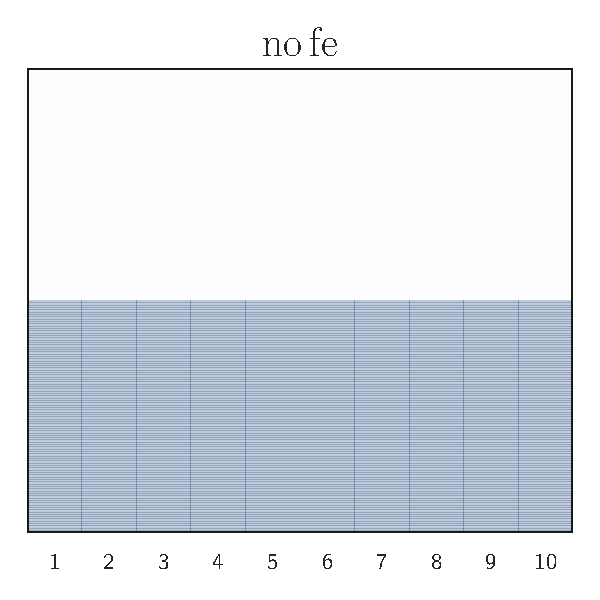
\includegraphics[width=1\linewidth]{plots/illustration/no-fe.pdf}
	\end{subfigure}%
	\begin{subfigure}{0.2\textwidth}
		\centering
		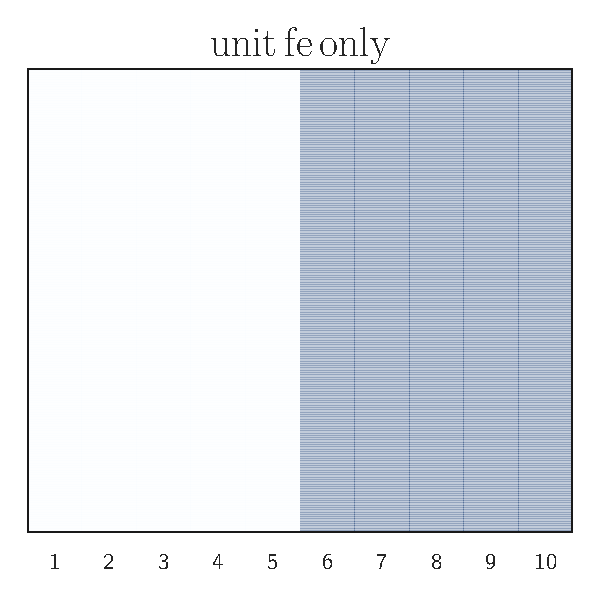
\includegraphics[width=1\linewidth]{plots/illustration/unit-fe.pdf}
	\end{subfigure}%
	\begin{subfigure}{0.2\textwidth}
		\centering
		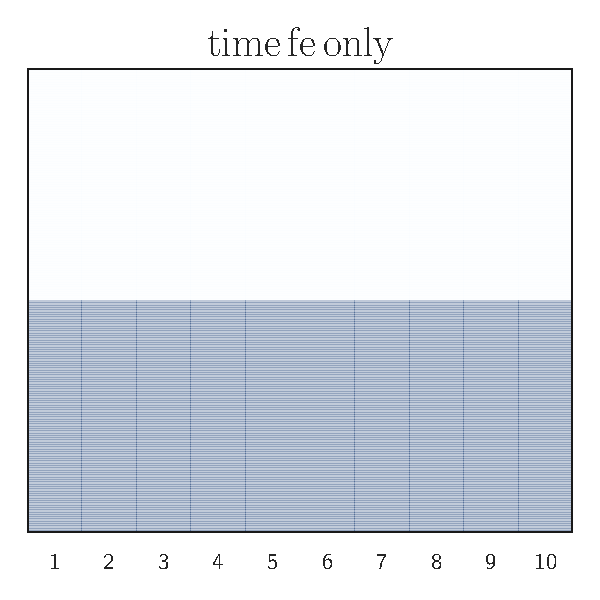
\includegraphics[width=1\linewidth]{plots/illustration/time-fe.pdf}
	\end{subfigure}%
	\begin{subfigure}{0.2\textwidth}
		\centering
		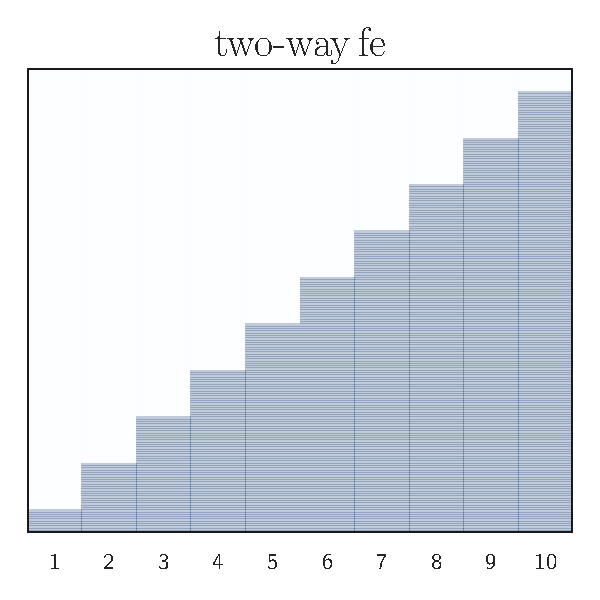
\includegraphics[width=1\linewidth]{plots/illustration/two-way-fe.pdf}
	\end{subfigure}%
	\begin{subfigure}{0.2\textwidth}
		\centering
		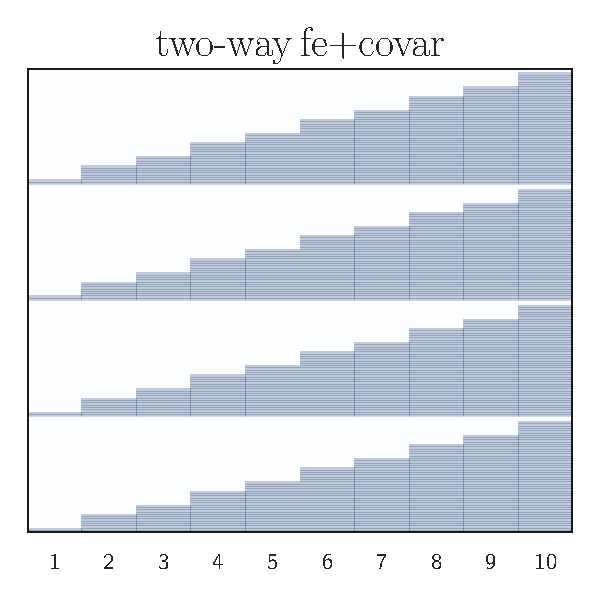
\includegraphics[width=1\linewidth]{plots/illustration/two-way-fe-covar.pdf}
	\end{subfigure}
	\caption{\textbf{Optimal treatment designs under various specifications.} Examples of T-optimal designs of $10$-period experiments with $\ell = 0$. Darker color denotes treatment, and lighter color denotes control. ``fe'' stands for ``fixed effects'' and ``covar'' stands for ``covariates''
	}
	\label{fig:various-optimal-design}
\end{figure}
	{\blue 
	
	To provide more intuition on the optimal treated fractions, we start with the specification with $\ell = 0$, and with either  $\alpha_i$ or $\beta_t$, but not both. 
	
	\begin{example}[Time Fixed Effects Only and $\ell = 0$]\label{example:time-only}
Suppose $Y_{it} = \beta_t + \tau_0 z_{it} + \varepsilon_{it}$ and Assumptions \ref{ass:treatment-adoption}, \ref{ass:model}, and \ref{ass:constant-error} hold. In this case,
$\mathrm{Prec}(\hat{\tau}_0)  = {N}/{\sigma_\varepsilon^2 } \cdot \big[T - \sum_{t=1}^T \omega_t^2  \big]$.
Any treatment design is optimal if it satisfies $\omega^\ast_t = 0$ for all $t$ and $z_{it} \leq z_{i,t+1}$ for all $i$ and $t$, that is, assigns treatment to 50\% units, while the others functioning as the control, for all time periods. 
\end{example}

\begin{example}[Unit Fixed Effects Only and $\ell = 0$]\label{example:unit-only}
Suppose	$Y_{it} = \alpha_i + \tau_0 z_{it} + \varepsilon_{it}$ and Assumptions \ref{ass:treatment-adoption}, \ref{ass:model}, and \ref{ass:constant-error} hold.  In this case,
$\mathrm{Prec}(\hat{\tau}_0) = {T}/{\sigma_\varepsilon^2 } \cdot \big[N - \sum_{i=1}^N \zeta_i^2 \big]$, 
where $\zeta_i = T^{-1} \sum_{t=1}^T z_{it}$.
Any treatment design is optimal if it satisfies $\omega^\ast_t = -1$ for all $t < (T+1)/2$ and $\omega^\ast_t = 1$ for all $t > (T+1)/2$, that is, allocates treatment to all units at halftime.\footnote{For odd $T$, units can be either treated or untreated at $t = (T+1)/2$.} 
\end{example}

    }


	If the specification has both $\alpha_i$ and $\beta_t$, as in Example \ref{example:two-way-fe}, 
	the optimal treated fractions are intuitively in between those in Examples \ref{example:time-only} and \ref{example:unit-only}. See Figure \ref{fig:various-optimal-design} for the visualization of optimal treated fractions under various specifications.


	
	The same intuition carries over to $\ell > 0$ and the precision matrix $\mathrm{Prec}(\hat{\bm{\tau}})$ is quadratic and concave in $\omega_t$. The two examples below provide the analytic expression of $\omega^\ast_{\ell,t}$ for $\ell = 1$ and $2$. We provide the expression of $\omega_{\ell,t}^\ast$ for $\ell = 3$ in Example \ref{remark:carryover-example-l3} of Section \ref{subsec:def-A-l-B-l}. 
	%
	

	
	\begin{example}[$\ell = 1$]\label{example:ell-1}
	In Theorem \ref{thm:obs-latent-carryover-model}, $\omega^\ast_{\ell,t}$ equals
		$-1 + {2(t-1)}/{(T-1)}$ for all $t$.
	\end{example}
%
	\begin{example}[$\ell = 2$]\label{example:ell-2}
	In Theorem \ref{thm:obs-latent-carryover-model}, $\omega^\ast_{\ell,t}$ is determined by, 
$\omega_{\ell,1}^\ast = -1$, $\omega_{\ell,2}^\ast = -1 + {2}/{(2T-5)}$, $\omega_{\ell,t}^\ast = -1 + {(2t-3)}/{(T-2)}$ for $t = 3, \cdots, T-2$, $\omega_{\ell,T-1}^\ast = 1 - {2}/{(2T-5)}$, and $\omega_{{\ell,T}}^\ast = 1$.
	\end{example}
	
    
    {\blue \paragraph{Intuition for the $S$-shaped curve of $\omega_{\ell,t}^\ast$.} The objective function in \eqref{eqn:obj} is a sum of $\ell+1$ quadratic functions, one function for each  $\mathrm{Prec}(\hat{\tau}_j)$ with $j \in \{0,1,\cdots,\ell\}$. Let $\omega_{\ell,t}^\ast(j)$ be the unit average of $z_{it}$ in the solution that maximizes $\mathrm{Prec}(\hat{\tau}_j)$ at time $t$, when the duration of lagged effects is $\ell$. This means $\omega^\ast_{\ell,t}$, defined in \eqref{eqn:omega-carryover}, can be written as a convex combination of $\omega_{\ell,t}^\ast(j)$ for all $j$ and $t$. Intuitively, since each $\omega_{\ell,t}^\ast(j)$ is chosen to maximize the precision of a single parameter $\hat{\tau}_j$, it should grow linearly in $t$, like the $\ell=0$ case, except during the first $\ell$ or the last $\ell$ periods that it is truncated to $0$ or $1$ respectively (see Figure \ref{fig:carryover-treatment-effect-t-opt-s-curve}). 
    Equipped with this observation, it is easy to see that $\omega^\ast_{\ell,t}$ grows linearly in $t$ in the middle (the third stage) where all $\omega^\ast_{\ell,t}$ grow linearly. $\omega^\ast_{\ell,t}$ is constant in stage one and five, where all $\omega^\ast_{\ell,t}$ are constant. Moreover, $\omega^\ast_{\ell,t}$ has a non-linear growth in stage two and four, because some of $\omega_{\ell,t}^\ast(j)$ are truncated to $0$ or $1$. 
    }
    
    \begin{figure}[t!]
		\centering
		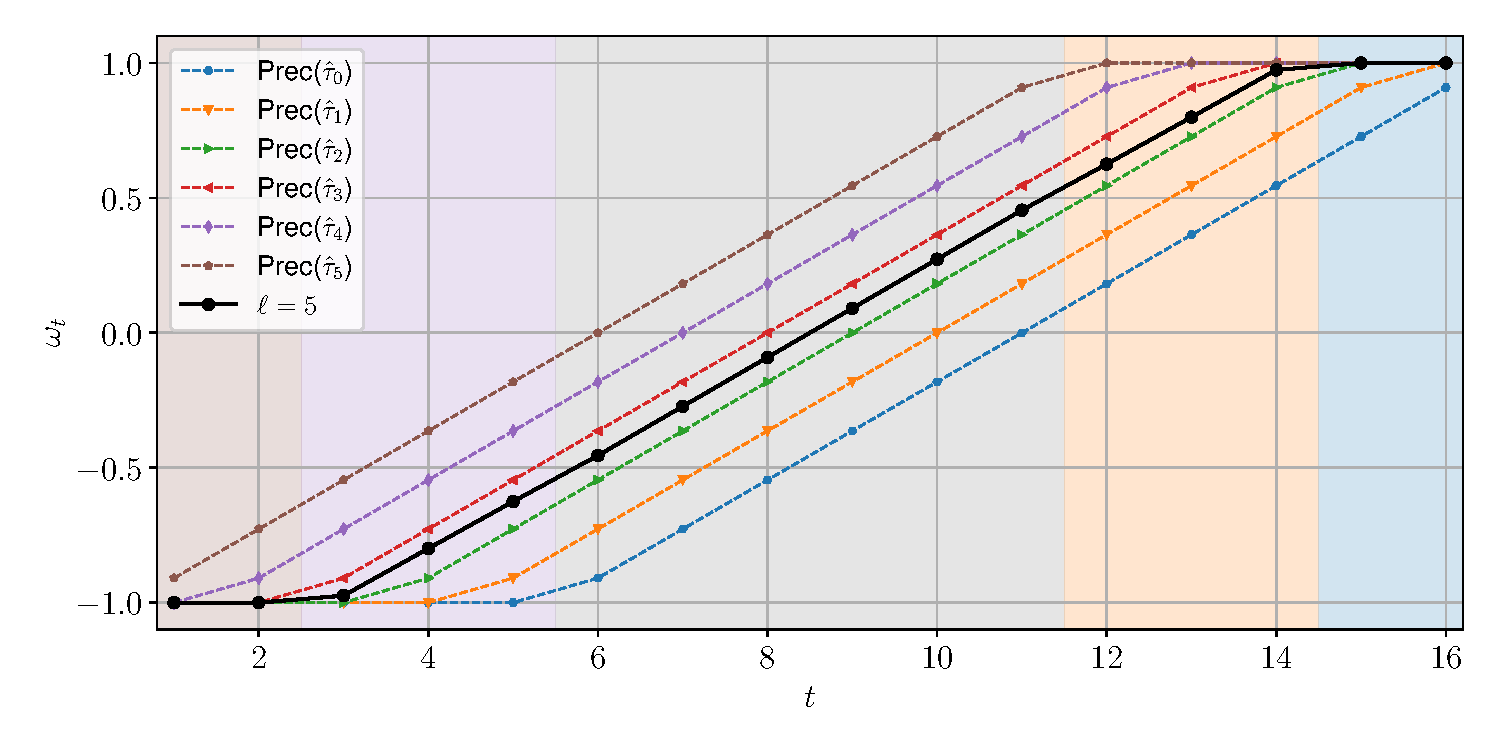
\includegraphics[width=0.5\linewidth]{plots/illustration/carryover-t-optimal-s-curve.pdf}
		\caption{Illustration of the $S$-shaped curve for the $ 16$-period optimal design with $\ell = 5$. For estimating $\tau_j$ only, the dashed lines denote the optimal $\omega_t$ that maximizes $\mathrm{Prec}(\hat{\tau}_j)$ for $j \in \{0,1,\cdots,5\}$. For estimating $\tau_0, \cdots, \tau_5$ simultaneously, the solid line denotes the optimal $\omega_t$ that maximizes $\mathrm{Prec}(\hat{\bm{\tau}})$, which is a convex combination of the dashed lines. The shaded regions from left to right denote the first to fifth stages in the solution $\omega^\ast_{\ell,t}$.  }
		\label{fig:carryover-treatment-effect-t-opt-s-curve}
	\end{figure}


	

	% \tocless
 \subsubsection{Choosing A Treatment Design}\label{subsec:choose-a-design}\texttt{}
	
	{\blue Based on the optimality conditions in Theorem \ref{thm:obs-latent-carryover-model}, we provide Algorithm \ref{algo:choose-design} in Section \ref{subsec:more-details-choose-design} to choose a treatment design.} In this subsection, we outline some general guidance on choosing a treatment design. When the specification does not have covariates ($d_x = d_u = 0$) and $\mathbb{A}_{\ell} $ is not empty, we can randomly choose one from $\mathbb{A}_\ell$ with equal probability. When the specification has observed, discrete-valued covariates ($d_x \neq 0$) and $\mathbb{A}^{\mathrm{disc}}_{\mathrm{opt}}$ is not empty, we can randomly choose one from $\mathbb{A}^{\mathrm{disc}}_\ell$ with equal probability. The random sampling can ensure that the treatment design balances the relevant covariates for the outcomes that are omitted in the specification \eqref{eqn:model-setup} and design of experiments \citep{hayes2017cluster}. 
	
	Note that $\mathbb{A}^{\mathrm{disc}}_{\mathrm{opt}}$ can be empty, if $|\tlo_g|(1+\omega_{\ell,t}^\ast)/(2T)$ is not an integer for each stratum (similarly for $\mathbb{A}_{\ell} $). For this case, Algorithm \ref{algo:choose-design} rounds $|\tlo_g|(1+\omega_{\ell,t}^\ast)/(2T)$ to the nearest integer to obtain a feasible design. As shown in Proposition \ref{prop:rounding-error-obs-cov} in Section \ref{subsubsec:practical-considerations}, the value of $\tr \big(\mathrm{Prec}(\hat{\bm{\tau}})  \big)$ evaluated at this feasible solution is within a factor of $1 + O \Lp {1}/{N^2} \Rp$ of the optimal value of $\tr \big(\mathrm{Prec}(\hat{\bm{\tau}})  \big)$.
	
	
	
	
	{\blue If observed covariates are continuous, then we can partition units into a small number of strata based on the observed covariate values, and then randomly choose a design that satisfies the treated fraction conditions for each stratum (possibly with rounding). Prior work has suggested keeping the number of strata small to avoid over-stratification \citep{kernan1999stratified}, because over-stratification may lower the precision of the estimated treatment effects \citep{de2008consequences}.  }
	
	
	{\blue If there are latent covariates, we suggest using the historical control data for the same set of units for the design of experiments. We can improve precision by using historical data to estimate $\*u_i$, partitioning units into strata ({\it e.g.}, by spectral clustering), and choosing a treatment design based on the estimated $\*u_i$. See Section \ref{subsec:latent-covariates} for more details. }
	
	
	\begin{remark}[Conditional Average Treatment Effect (CATE)]\label{remark:cate}
	Suppose we are interested in using observable sources of heterogeneity $\*X_i$ to assess the heterogeneity in treatment effects (\cite{robinson1988root,wager2018estimation} among others). In this case, we may be interested in conditional average instantaneous and lagged effects, denoted by $\tau_j(\*X_i)$. If $\*X_i$ is discrete, the designs satisfying \eqref{eqn:opt-finite-x-interactive-effect-carryover} can maximize the precision of $\hat{\tau}_j(\*X_i)$ for all $j$ and $\*X_i$, following that the optimality conditions for $\omega_{\ell,t}^\ast$ are satisfied within each stratum.
    
	\end{remark}
	

	

    
    {\blue \begin{remark}[Discussion on Adaptive Design]\label{rem:fixed-sample-adaptive-design}
	The treatment assignments studied in this section are chosen and fixed before the experiment starts. For non-adaptive experiments, we do not pursue adaptive designs, where treatment assignments for subsequent periods can vary during the experiment, for the following reason. From Theorem \ref{thm:obs-latent-carryover-model}, the information that matters for the treatment assignments but is unknown before the experiment starts is $\*u_i$. However, the estimation of $\*u_i$ at the beginning of the experiment can be quite noisy, and we do not expect noisy estimates of $\*u_i$ can substantially help the design. See Section \ref{subsubsec:choose-treatment-design} for further elaboration on this.
\end{remark}}